\section{协同推理机制验证}
\label{sec:system_validation}

本节检验黑板调度下的协同推理机制能否稳定支撑多轮求解过程。验证重点放在三个方面：共享黑板是否能够减少状态漂移，共享缓存是否能够支撑失败回放和恢复，错误归因与预算控制是否能够降低无效重试。围绕这些问题，本文从重复运行稳定性、检索信号质量、参数预算、运行开销、鲁棒性和消融实验等方面展开验证。

\subsection{重复运行稳定性分析}

对于多智能体图推理系统而言，单次精确匹配率只能反映最终答案是否正确，还需要考察多次运行时结果是否稳定，以及候选程序在失败后能否在限定轮数内收敛。因此，本文从不同运行轮次之间的精确匹配率波动范围、程序首次生成即通过验证的比例，以及进入修复循环后能够在限定轮数内收敛的比例三个角度进行统计，结果如表\ref{tab:stability_observation}所示。

\begin{table}[htbp]
\centering
\caption{重复运行中的稳定性观察（\%）}
\label{tab:stability_observation}
\begin{tabular}{lccc}
\toprule
数据集 & 精确匹配率波动范围 & 首次通过率 & 修复后收敛率 \\
\midrule
GraphArena & $\pm0.7$ & 79.6 & 91.4 \\
NLGraph & \textbf{$\pm0.5$} & \textbf{82.3} & \textbf{93.1} \\
GraphWiz & $\pm0.9$ & 74.8 & 89.7 \\
\bottomrule
\end{tabular}
\end{table}

表\ref{tab:stability_observation}显示，结构较清晰、标准算法映射较稳定的任务在三个指标上整体更优；约束更复杂的任务首次通过率略低，但经过反馈修复后仍能保持较高收敛水平。该结果说明，PlanGraph 的协同推理机制除了提高单次运行的精确匹配率，还能抑制多次运行时的结果波动，并对失败样例提供有限恢复能力。黑板事件和共享缓存链为这些统计提供了直接依据：每次失败、修复和重新验证都被记录为可追踪事件，因此可以区分首次成功、修复成功和最终失败三类情况。

\subsection{检索质量验证}

为了更细致地验证共享黑板中的规划状态和结构约束标签是否能改善检索智能体的输入质量，本文比较四种查询方式：直接使用原始问题文本进行检索、使用任务类型和关键词进行简化检索、使用规划伪代码进行检索，以及在规划伪代码基础上补充结构约束标签进行检索。实验基于五个基准测试集构造对应查询实例，统计 Hit@1、Hit@3、Hit@5 以及平均倒数排名（MRR）四项指标，结果如表\ref{tab:retrieval_quality}所示。

\begin{table}[htbp]
\centering
\caption{不同检索查询方式的知识命中效果对比}
\label{tab:retrieval_quality}
\begin{tabular}{lcccc}
\toprule
查询方式 & Hit@1 & Hit@3 & Hit@5 & MRR \\
\midrule
Q1 原始问题文本 & 42.6\% & 61.8\% & 72.9\% & 51.4\% \\
Q2 任务类型和关键词 & 68.9\% & 84.7\% & 92.1\% & 76.3\% \\
Q3 规划伪代码 & 76.4\% & 90.8\% & 96.3\% & 83.5\% \\
Q4 规划伪代码及结构约束标签 & \textbf{82.1\%} & \textbf{94.2\%} & \textbf{98.0\%} & \textbf{88.4\%} \\
\bottomrule
\end{tabular}
\end{table}

从表\ref{tab:retrieval_quality}可见，四种查询方式呈现出清晰的层次关系：直接使用原始问题文本的效果最弱；在显式加入任务语义后，Q2 的命中效果明显提升；将问题压缩为规划伪代码后，Q3 在四项指标上继续改善；当查询中继续补充图类型、目标形式和关键约束等结构化标签时，Q4 的检索排序质量达到最好。Q3 和 Q4 在 MRR 上的提升还说明，黑板中保存的规划状态会影响正确知识的召回情况和排序位置，从而有助于减少编码阶段对错误 API 或不相关文档的尝试次数。这一结果从实验上支持了共享状态约束检索输入的协同推理机制。

\subsection{参数敏感性分析}

为观察检索返回条数和修复轮数对协同恢复过程的影响，本文比较六组代表性参数组合，即 $(1,0)$、$(3,1)$、$(5,3)$、$(7,3)$、$(5,4)$ 和 $(9,4)$。其中，$k$ 表示检索模块返回的候选知识条目数，$r$ 表示最大反馈修复轮数。该实验选取具有稳定难度分层的典型组合优化任务子集，重点比较简单样本与困难样本两个端点，并统计子集精确匹配率、难度分层精确匹配率、执行成功率、平均修复轮数与平均端到端耗时。该处数值用于分析预算约束和恢复深度，不对应第五章完整基准集合上的总体精确匹配率。

\begin{table}[htbp]
\centering
\caption{不同参数组合下典型组合优化子集的性能比较（\%）}
\label{tab:param_main_result}
\small
\resizebox{\textwidth}{!}{%
\begin{tabular}{lcccccccc}
\toprule
$(k,r)$ & 子集 EM & 简单样本 EM & 困难样本 EM & 执行成功率 & 平均修复轮数 & 平均耗时(s) & $\Delta$EM vs $(3,1)$ & $\Delta$耗时(s) vs $(3,1)$ \\
\midrule
$(1,0)$ & 70.00 & \textbf{85.00} & 55.00 & 74.20 & \textbf{0.00} & \textbf{13.80} & -4.17 & -1.40 \\
$(3,1)$ & \textbf{74.17} & 82.50 & 63.75 & 80.80 & 0.36 & 15.20 & 0.00 & 0.00 \\
$(5,3)$ & 68.75 & 75.00 & 61.25 & 78.30 & 0.92 & 18.40 & -5.42 & +3.20 \\
$(7,3)$ & 73.75 & 80.00 & \textbf{66.25} & \textbf{81.70} & 0.88 & 17.60 & -0.42 & +2.40 \\
$(5,4)$ & 71.25 & 75.00 & 65.00 & 80.40 & 1.14 & 20.90 & -2.92 & +5.70 \\
$(9,4)$ & 71.25 & 77.50 & 63.75 & 79.20 & 1.20 & 19.70 & -2.92 & +4.50 \\
\bottomrule
\end{tabular}
}
\end{table}

表\ref{tab:param_main_result}显示，$r=0$ 时 PlanGraph 缺少反馈修复能力，困难样本精确匹配率下降到 55.00\%；当参数增大到 $(7,3)$、$(5,4)$ 或 $(9,4)$ 时，更多知识条目和修复轮数未带来稳定的子集收益。相比之下，$(3,1)$ 能够在保持较高子集精确匹配率的同时控制平均修复轮数和平均耗时，说明适中的检索规模与少量反馈修复更适合作为默认配置，也说明有界恢复比无约束增加修复轮数更符合协同调度目标。

\subsection{运行开销分析}

为了说明 PlanGraph 的运行代价，本文统计了其在典型任务上的平均端到端推理耗时、平均代码生成轮数和平均验证次数。这里选取三类代表任务：最短路径、最大流和旅行商问题。平均耗时会受到模型接口响应、返回长度与验证轮次等因素影响，因此表\ref{tab:efficiency}中的数值主要用于展示本系统在不同任务之间的相对开销差异。

\begin{table}[htbp]
\centering
\caption{不同任务上的平均推理开销}
\label{tab:efficiency}
\begin{tabular}{lccc}
\toprule
任务类型 & 平均耗时（s） & 平均生成轮数 & 平均验证次数 \\
\midrule
最短路径 & \textbf{10.8} & \textbf{1.1} & \textbf{1.3} \\
最大流 & 14.6 & 1.3 & 1.8 \\
旅行商问题 & 24.3 & 1.8 & 2.7 \\
\bottomrule
\end{tabular}
\end{table}

表\ref{tab:efficiency}显示，不同任务的运行开销差异较明显。最短路径问题结构相对清楚，算法接口也较成熟，因此规划、检索和验证过程通常较为顺畅。最大流任务需要处理容量约束和残量网络，程序实现中涉及的状态更新更多，平均验证次数因此有所增加。旅行商问题还需要显式处理组合搜索、节点覆盖、回路闭合和可行性判断，因而整体耗时和验证次数最高。就本文研究目标而言，更强调可靠地完成图推理，而非追求最低时延响应，因此以一定推理开销换取更高精确匹配率和结果可信度是合理的设计选择。

\subsection{鲁棒性消融分析}

除标准基准测试集外，本文还在输入扰动设置下考察 PlanGraph 的表现，以分析框架对问题表述变化的稳定性。该实验覆盖五个基准测试集，并构造三种常见扰动：节点顺序随机打乱、边列表描述改写、输出要求从自然语言答案改为结构化列表。在相同求解任务下比较精确匹配率变化，结果如表\ref{tab:robustness}所示。

\begin{table}[htbp]
\centering
\caption{输入扰动条件下的鲁棒性分析（\%）}
\label{tab:robustness}
\begin{tabular}{lccc}
\toprule
扰动类型 & GPT-4o & GraphTeam & PlanGraph \\
\midrule
节点顺序打乱 & 51.6 & 92.4 & \textbf{96.8} \\
边描述改写 & 48.9 & 91.1 & \textbf{95.7} \\
输出格式切换 & 44.3 & 89.8 & \textbf{94.9} \\
\bottomrule
\end{tabular}
\end{table}

表\ref{tab:robustness}显示，PlanGraph 在输入扰动下仍然保持较高精确匹配率。本文认为其原因在于：问题智能体先将自然语言输入规整为结构化表示，减少了不同表述形式对后续规划的影响；程序执行结果在最终答案生成前还会经过格式化处理，因此输出形式变化对系统影响相对有限。

为判断关键协同组成是否具有必要性，本文设计三种消融变体：（1）去除规划模块，直接根据原始问题生成代码；（2）去除检索模块，移除规划引导检索，仅依赖模型内部知识生成程序；（3）去除验证模块，移除程序执行验证与反馈修复闭环，仅保留一次性代码生成。图\ref{fig:ablation_result_visual}给出了在三个代表性数据集上的消融结果。

\begin{figure}[htbp]
\centering
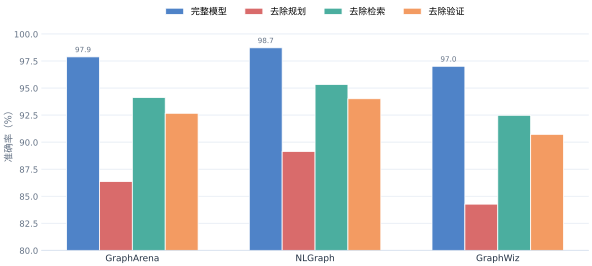
\includegraphics[width=0.90\textwidth]{figures/paper/exp_ablation.pdf}
\caption{关键协同组成消融实验结果}
\label{fig:ablation_result_visual}
\end{figure}

图\ref{fig:ablation_result_visual}显示，移除规划模块后，三个数据集上的结果都出现了最明显的下降，说明规划模块是 PlanGraph 中较关键的组成部分。去除验证模块后，系统性能也出现了较大下降，尤其在 GraphWiz 上从 97.01\% 降至 90.72\%。检索模块带来的性能提升相对温和，但依然稳定。规划模块约束任务目标与求解方向，检索模块补充实现依据，验证模块检查结果是否满足要求，三类组成形成 PlanGraph 的协同闭环。

\subsection{提示词查询模板复现说明}

为保证系统可复现性，本文将各智能体提示词和检索查询模板设计为相对固定的结构化模板。问题智能体用于将原始自然语言问题解析为结构化图推理任务，输出字段包括 \texttt{task\_type}、\texttt{nodes}、\texttt{edges}、\texttt{directed}、\texttt{weighted}、\texttt{capacity}、\texttt{params}、\texttt{output\_format} 和 \texttt{constraints}。规划智能体用于生成算法级伪代码规划，并为检索阶段提供算法提示、约束标签和检索术语。编码智能体基于任务、规划和检索知识生成可执行 Python 程序，并要求使用标准库和 NetworkX 完成图结构建模和算法调用。推理智能体则根据执行反馈和检索反馈修正当前程序，主要处理图构建错误、API 使用错误、约束遗漏和输出格式不匹配等问题。

检索智能体根据规划结果和反馈信息组织检索查询，不生成自然语言回答。其查询构造主要利用任务类型、图属性、算法提示、约束标签、输出格式以及执行错误信息。表\ref{tab:retrieval_query_template}给出了检索查询模板摘要。

\begin{table}[htbp]
\centering
\small
\caption{检索查询模板摘要}
\label{tab:retrieval_query_template}
\begin{tabular}{p{2.0cm}p{10.5cm}}
\toprule
查询类型 & 构造依据 \\
\midrule
\texttt{Q0} & \texttt{task\_type and graph attributes} \\
\texttt{Q1} & \texttt{key actions from pseudocode and algorithm\_hints} \\
\texttt{Q2} & \texttt{constraint\_tags and output\_format} \\
\texttt{Q3} & \texttt{retrieval gaps or low-coverage constraints} \\
\texttt{Q4} & \texttt{execution error type, failed API, and repair target} \\
\texttt{Ranking} & \texttt{semantic relevance, task-tag matching, and constraint consistency} \\
\bottomrule
\end{tabular}
\end{table}

上述模板避免暴露模型内部不可控推理链，并要求各阶段返回可检查的阶段结果。通过固定字段、固定查询类型和统一输出格式，PlanGraph 能够在批量实验中保持较一致的运行条件，也便于对失败样例进行回放和复核。
